\subsection{Redovno javljanje}

Redovno javljanje predstavlja postupak vo\dj enja redovne evidencije teku\' ceg stanja nezaposlenog lica u Nacionalnoj slu\v zbi. Nezaposleno lice je u obavezi da se na svaka 3 meseca javi u Nacionalnoj slu\v zbi, i da izvesti zaposlene koji posreduju u zapo\v sljavanju o svom trenutnom statusu.\\

U zavisnosti od nivoa izve\v stavanja nezaposleno lice mo\v ze da bira na\v cin redovnog javljanja, i to (Slika \ref{dsu: redovno javljanje}):
\begin{itemize}
	\item ukoliko nema potrebu za dodatnim uslugama Nacionalne slu\v zbe, bira jedno od naredna dva:
	\begin{itemize}
		\item Javljanje putem interneta (slu\v caj upotrebe \ref{su: javljanje putem interneta}), ili
		\item Javljanje na \v salteru (slu\v caj upotrebe \ref{su: javljanje na salteru}).
	\end{itemize}
	
	\item ukoliko ima potrebu za dodatnim uslugama Nacionalne slu\v zbe, onda bira Javljanje kod savetnika (slu\v caj upotrebe \ref{su: javljanje kod savetnika}).
\end{itemize}

\begin{figure}[H]
	\centering
	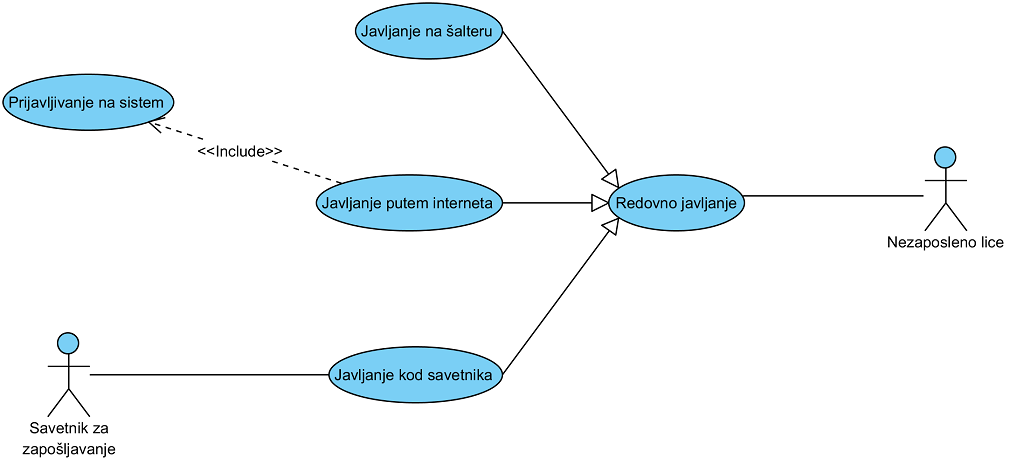
\includegraphics[width=\textwidth]{dijagrami/dijagrami-slucajeva-upotrebe/redovno-javljanje.png}
	\caption{Dijagram slu\v cajeva upotrebe procesa ''Redovno javljanje''.}
	\label{dsu: redovno javljanje}
\end{figure}

Unapre\dj enje trenutnog re\v senja predstavlja Javljanje putem interneta. Ovim slu\v cajem upotrebe se uvodi novi deo onlajn sistema Nacionalne slu\v zbe, radi olak\v savanja procesa Redovno Javljanje nezaposlenih lica koji nemaju dodatne potrebe za uslugama Nacionalne slu\v zbe. Doprinosi ovog unapre\dj enja su:
\begin{itemize}
	\item smanjenje reda \v cekanja u Nacionalnoj slu\v zbi,
	\item usmeravanje rada \v salterskog slu\v zbenika na druge (zna\v cajnije) radne aktivnosti i zadatke, i
	\item obavljanje procesa Redovno javljanje iz komfornosti doma.
\end{itemize}

\subsubsection{Javljanje putem interneta}
\label{su: javljanje putem interneta}

\noindent U\v cesnici: Nezaposleno lice (u daljem tekstu NL)
\\
\\ Preduslovi: NL ima otvoren nalog u onlajn sistemu.
\\
\\ Postuslovi: Ili je uspe\v sno zabele\v zeno javljanje NL-a ili je NL obave\v sten o svom stanju.
\\ 
\\ Glavni tok:
\begin{enumerate}
	\item NL pristupa onlajn sistemu Nacionalne slu\v zbe.
	\item Sistem prikazuje formular za prijavljivanje na sistem.
	\item Prelazi se na slu\v caj upotrebe \ref{su: prijavljivanje na sistem}.
	\begin{enumerate}
		\item U slu\v caju uspe\v snog prijavljivanja na sistem, sistem prikazuje po\v cetni interfejs NL-u, i prelazi se na korak 4.
		\item Ina\v ce, sistem prikazuje poruku NL-u i slu\v caj upotrebe se zavr\v sava.
	\end{enumerate}
	\item NL bira opciju ``Redovno javljanje''.
	\item NL bira da li \v zeli da zaka\v ze sastanak sa savetnikom za zapo\v sljavanje ili ne.
	\item NL bira da zaka\v ze sastanak.
	\begin{enumerate}
		\item Sistem pronalazi savetnika za zapo\v sljavanje koji je zadu\v zen za NL.
		\item Sistem zakazuje prvi slobodni termin za sastanak.
		\item Sistem prikazuje NL-u zakazani termin.
		\item NL potvr\dj uje izbor, i prelazi se na korak 8.
	\end{enumerate}
	\item NL bira da ne zaka\v ze sastanak, pa se prelazi na korak 8.
	\item Sistem bele\v zi da je NL uspe\v sno obavio proceduru.
	\item Sistem bele\v zi da \v salterski slu\v zbenik treba da upi\v se datume i stavi potpis u evidencioni karton NL-a kada NL slede\'ci put do\dj e u Nacionalnu slu\v zbu.
\end{enumerate}

\noindent Alternativni tokovi: 
\\/

\subsubsection{Javljanje na \v salteru}
\label{su: javljanje na salteru}

\noindent U\v cesnici: Nezaposleno lice (u daljem tekstu NL), \v salterski slu\v zbenik (u daljem tekstu \v SS)
\\
\\ Preduslovi: NL ima evidentacioni karton. \v SS je ulogovan na sistem. 
\\
\\ Postuslovi: Ili je uspe\v sno zabele\v zeno javljanje NL-a ili je NL obave\v sten o svom stanju.
\\ 
\\ Glavni tok:
\begin{enumerate}
	\item NL prilazi automatu i bira opciju ''Redovno javljanje''.
	\item Automat bele\v zi da je opcija ''Redovno javljanje'' odabrana, ra\v cuna naredni broj u redu \v cekanja za tu opciju, i \v stampa papir sa brojem.
	\item NL uzima broj i \v ceka svoj red.
	\item Kada do\dj e na red, NL prilazi \v salteru, zahteva od \v SS da prijavi njegov dolazak, i predaje \v SS-u svoj evidentacioni karton.
	\item \v SS pronalazi NL-a u sistemu.
	\item \v SS unosi u sistem da je NL do\v sao na redovno javljanje.
	\item \v SS zakazuje slede\' ce javljanje i vra\' ca NL-u evidentacioni karton.
\end{enumerate}

\noindent Alternativni tokovi: 
\begin{description}
	\item[A1. Pad sistema] ~\\
	Ukoliko se u bilo kom koraku Glavnog toka dogodi pad sistema na kojem radi \v SS, \v SS ponovo pokre\'ce sistem i prijavljuje se na njega. Prelazi se na korak 5 Glavnog toka.
	
	\item[A2. Status NL-a je ''zamrznut''] ~\\
	Ukoliko u koraku 5 Glavnog toka sistem prika\v ze da je status NL-a ''zamrznut'', \v SS obave\v stava NL-a o njegovom statusu, i slu\v caj upotrebe se zavr\v sava.
\end{description}

\subsubsection{Javljanje kod savetnika}
\label{su: javljanje kod savetnika}

\noindent U\v cesnici: Nezaposleno lice (u daljem tekstu NL), savetnik za zapo\v sljavanje (SZ)
\\
\\ Preduslovi: NL ima evidentacioni karton. SZ je ulogovan na sistem. 
\\
\\ Postuslovi: Ili su podaci o NL-u izmenjeni ili su podaci ostali nepromenjeni ili je NL obave\v sten o svom stanju.
\\ 
\\ Glavni tok:
\begin{enumerate}
	\item NL dolazi kod SZ u kancelariju i predaje mu svoj evidentacioni karton.
	\item SZ pronalazi NL u sistemu.
	\item SZ i NL razgovaraju o ve\v stinama koje je NL stekao od poslednjeg javljanja.
	\item SZ unosi nove informacije u sistem.
	\item SZ tra\v zi informacije o poslovima koje mogu da zanimaju NL.
	\item Sistem ispisuje informacije o takvim poslovima. 
	\item SZ nudi teku\' ci posao NL.
	\item SZ i NL razgovaraju o teku\' cem poslu.
	\item SZ nudi NL da zaka\v ze razgovor za posao.
	\item NL bira da ugovori razgovor za posao.
	\begin{enumerate}
		\item SZ unosi potrebne podatke u sistem.
		\item Sistem, zajedno sa informacionim sistemom kompanije, zakazuje razgovor za posao, a zatim isporu\v cuje informacije SZ.
		\item SZ obave\v stava NL o isporu\v cenim informacijama.
		\item Prelazi se na korak 12.
	\end{enumerate}
	\item NL bira da ne ugovori razgovor za posao, pa se prelazi na korak 12.
	\item Koraci 7 do 9 se ponavljaju sve dok ima poslova u ponudi.
	\item SZ zakazuje slede\' ce javljanje i vra\' ca NL-u evidentacioni karton.
\end{enumerate}

\noindent Alternativni tokovi: 
\\/

\begin{mylandscape}
	\subsubsection{BPMN dijagrami}
	
	\begin{figure}[H]
		\centering
		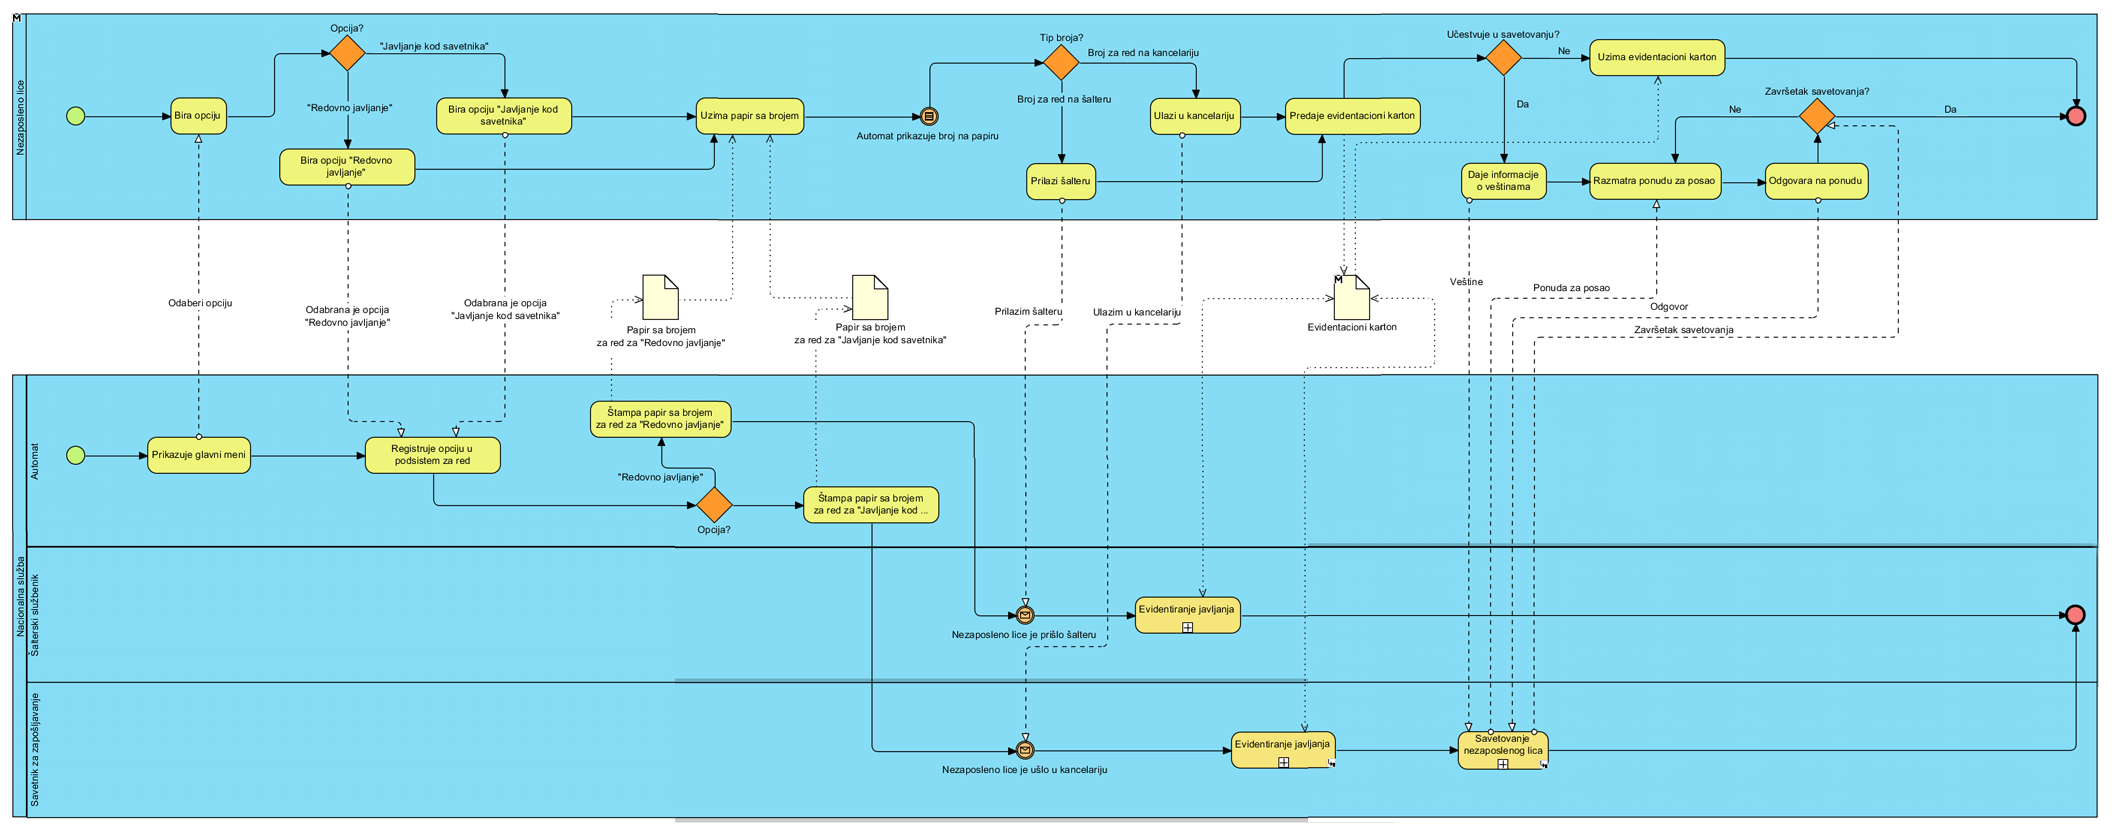
\includegraphics[width=0.8\paperwidth]{dijagrami/bpmn-dijagrami/redovno-javljanje-bpmn.png}
		\caption{BPMN dijagram procesa ''Redovno javljanje'' (bez ''Javljanje putem interneta'').}
		\label{bpmnd: redovno javljanje}
	\end{figure}

	\newpage
	
	\begin{figure}[H]
		\centering
		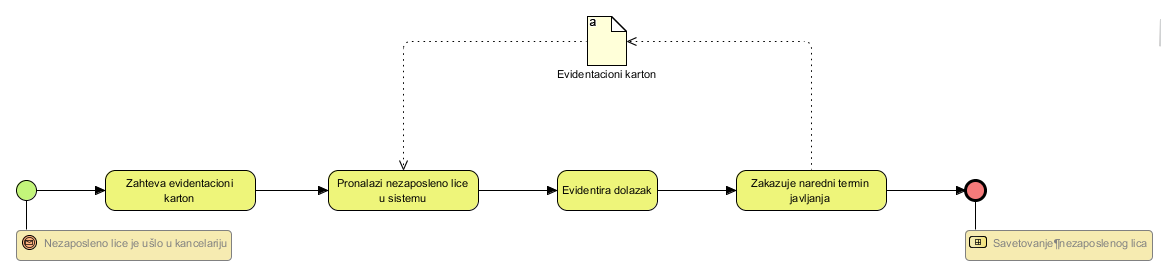
\includegraphics[width=0.8\paperwidth]{dijagrami/bpmn-dijagrami/evidentiranje-javljanja.png}
		\caption{BPMN dijagram potprocesa ''Evidentiranje javljanja'' procesa ''Redovno javljanje'' (Slika \ref{bpmnd: redovno javljanje}).}
	\end{figure}

	\newpage
	
	\begin{figure}[H]
		\centering
		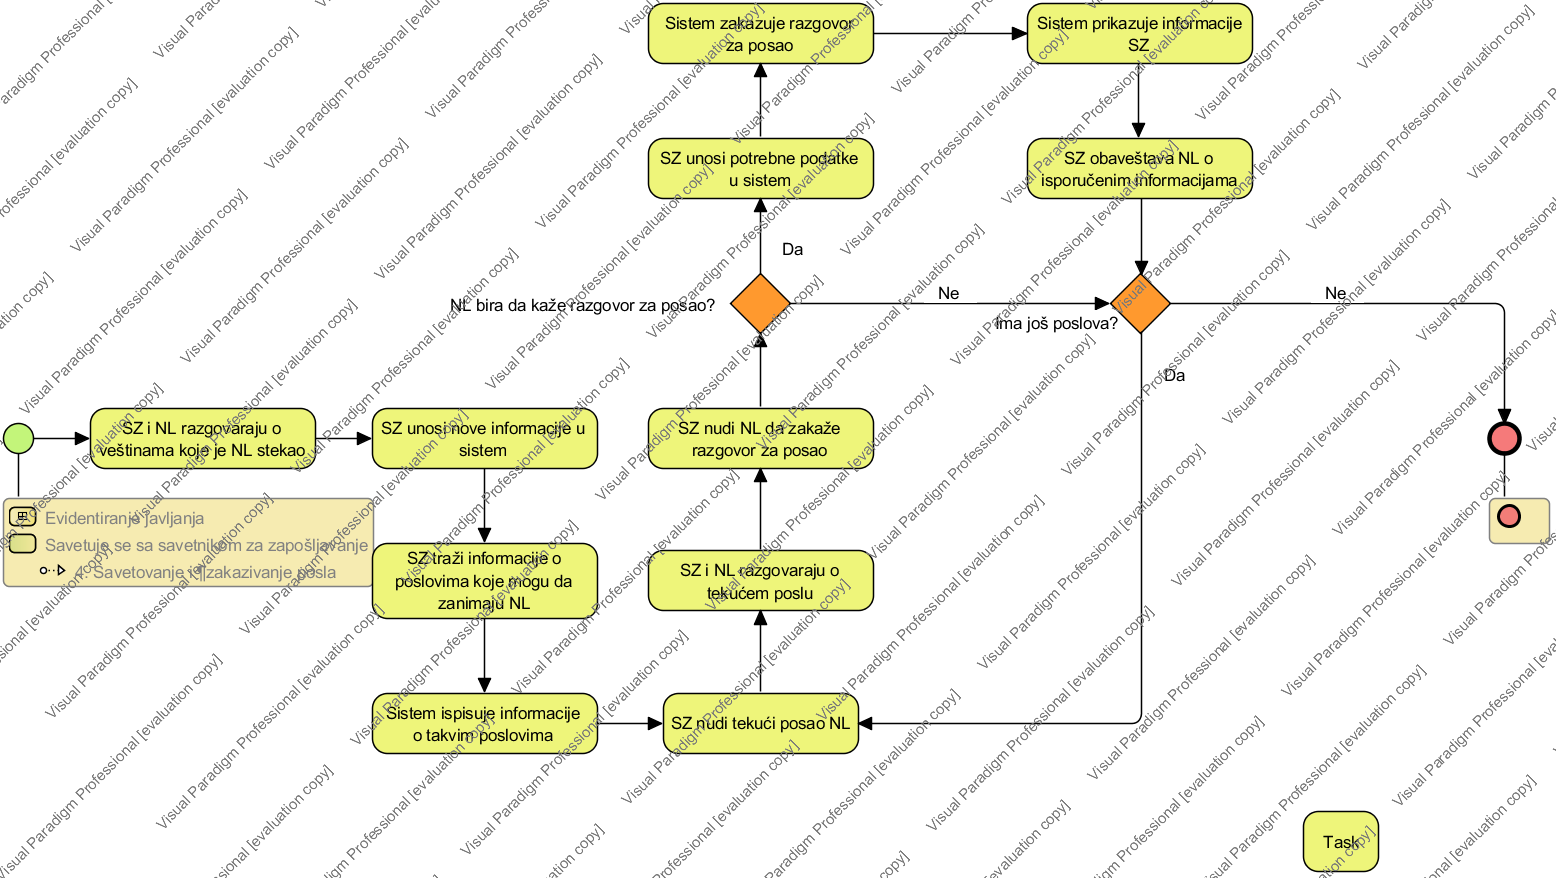
\includegraphics[width=0.8\paperwidth]{dijagrami/bpmn-dijagrami/savetovanje-nezaposlenog-lica.png}
		\caption{BPMN dijagram potprocesa ''Savetovanje nezaposlenog lica'' procesa ''Redovno javljanje'' (Slika \ref{bpmnd: redovno javljanje}).}
	\end{figure}
\end{mylandscape}